\subsection{Using Different Template Meshes}
\label{ch3:sec:discussion_different_mesh}

We found that the auto-decoder trained with TM-A works well on other types of template mesh, even without additional adaptations after training.
It means that, given a different template mesh $\Tilde{M}=\{\Tilde{V}, \Tilde{E}\}$ and the auto-decoder $g_\Theta*$ trained with template mesh $\hat{M}$, we can still well solve
%
\begin{align}
    \bz^* &=  \argmin_{\bz} \cL(\Tilde{M}(\Tilde{\bv} + g_{\Theta^*}(\bz, \Tilde{M})) , S) \; .
\end{align}
%
To test he model's generalization ability, we use four different template meshes.

\begin{figure}[!tb]
	\begin{center}
		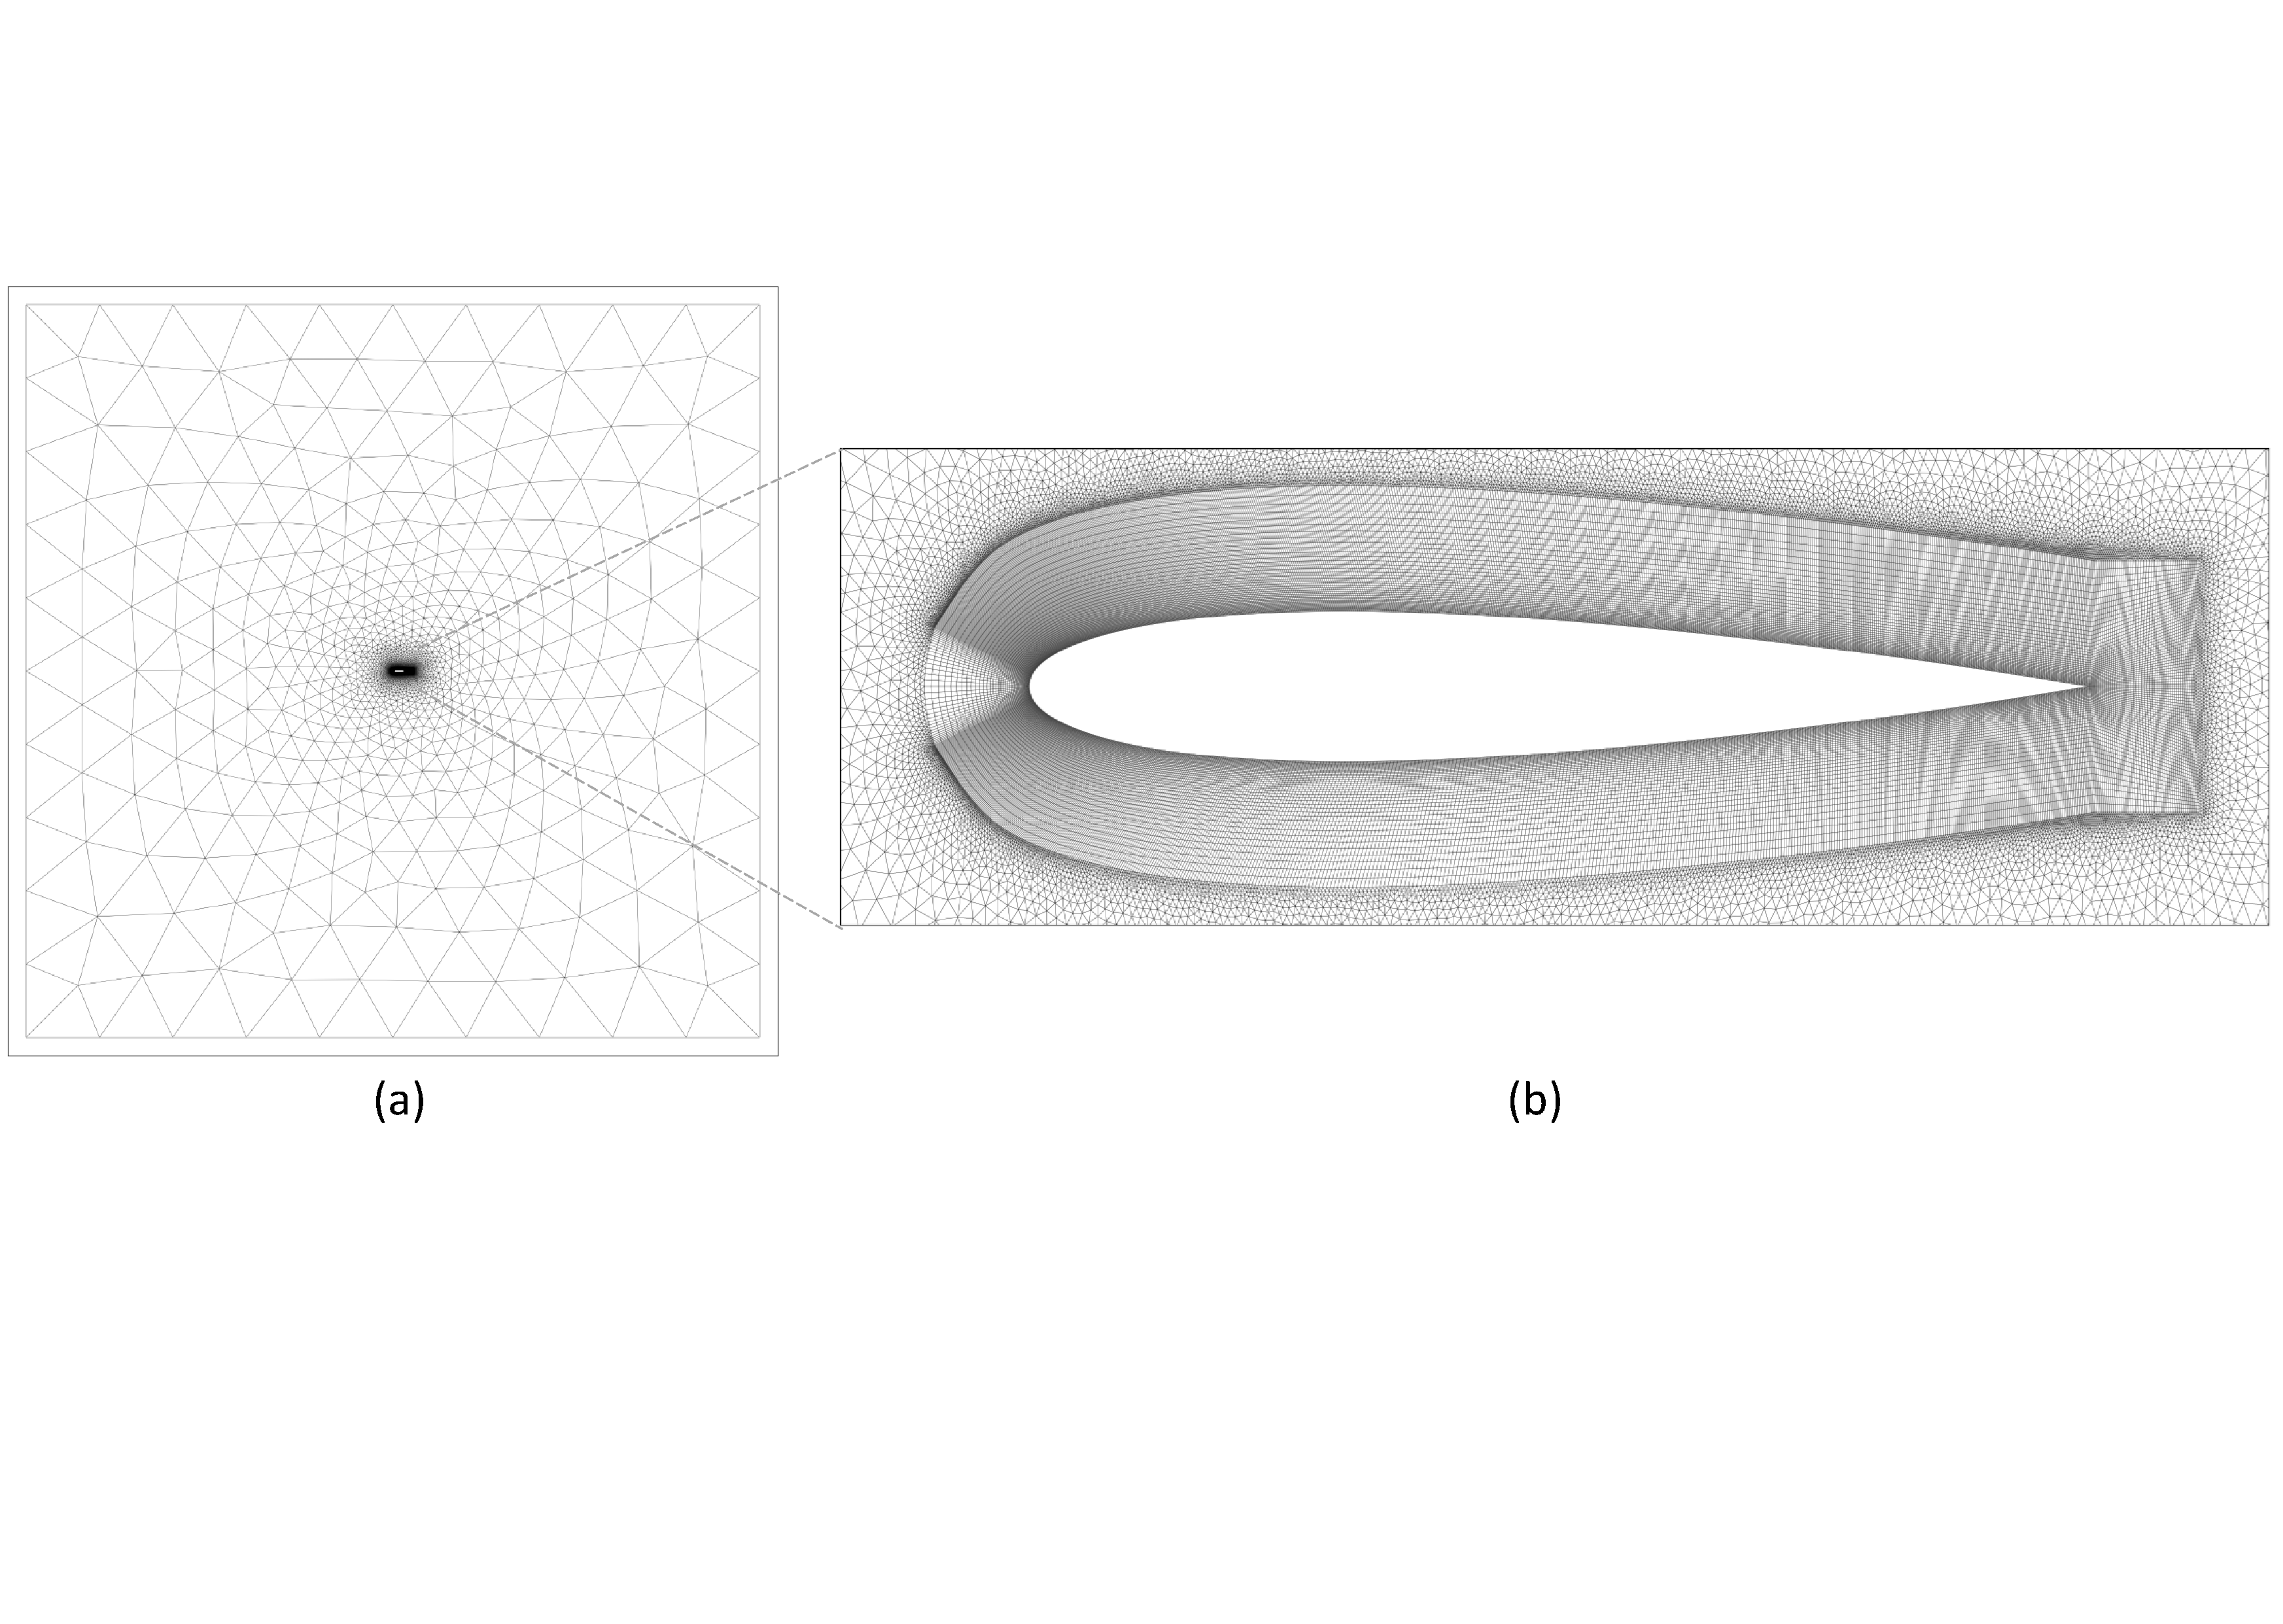
\includegraphics[width=1\linewidth]{chapter3/tex/figures/experiment/init_template_mesh_vlab.pdf}
	\end{center}
	\caption{ \small
		The hybrid parametric template mesh (TM-B) with (a) an overall and (b) a zoomed-in views.
	}
	\label{ch3:fig:discuss_init_vlab_mesh}
\end{figure}

\begin{figure}[!htb]
	\begin{center}
		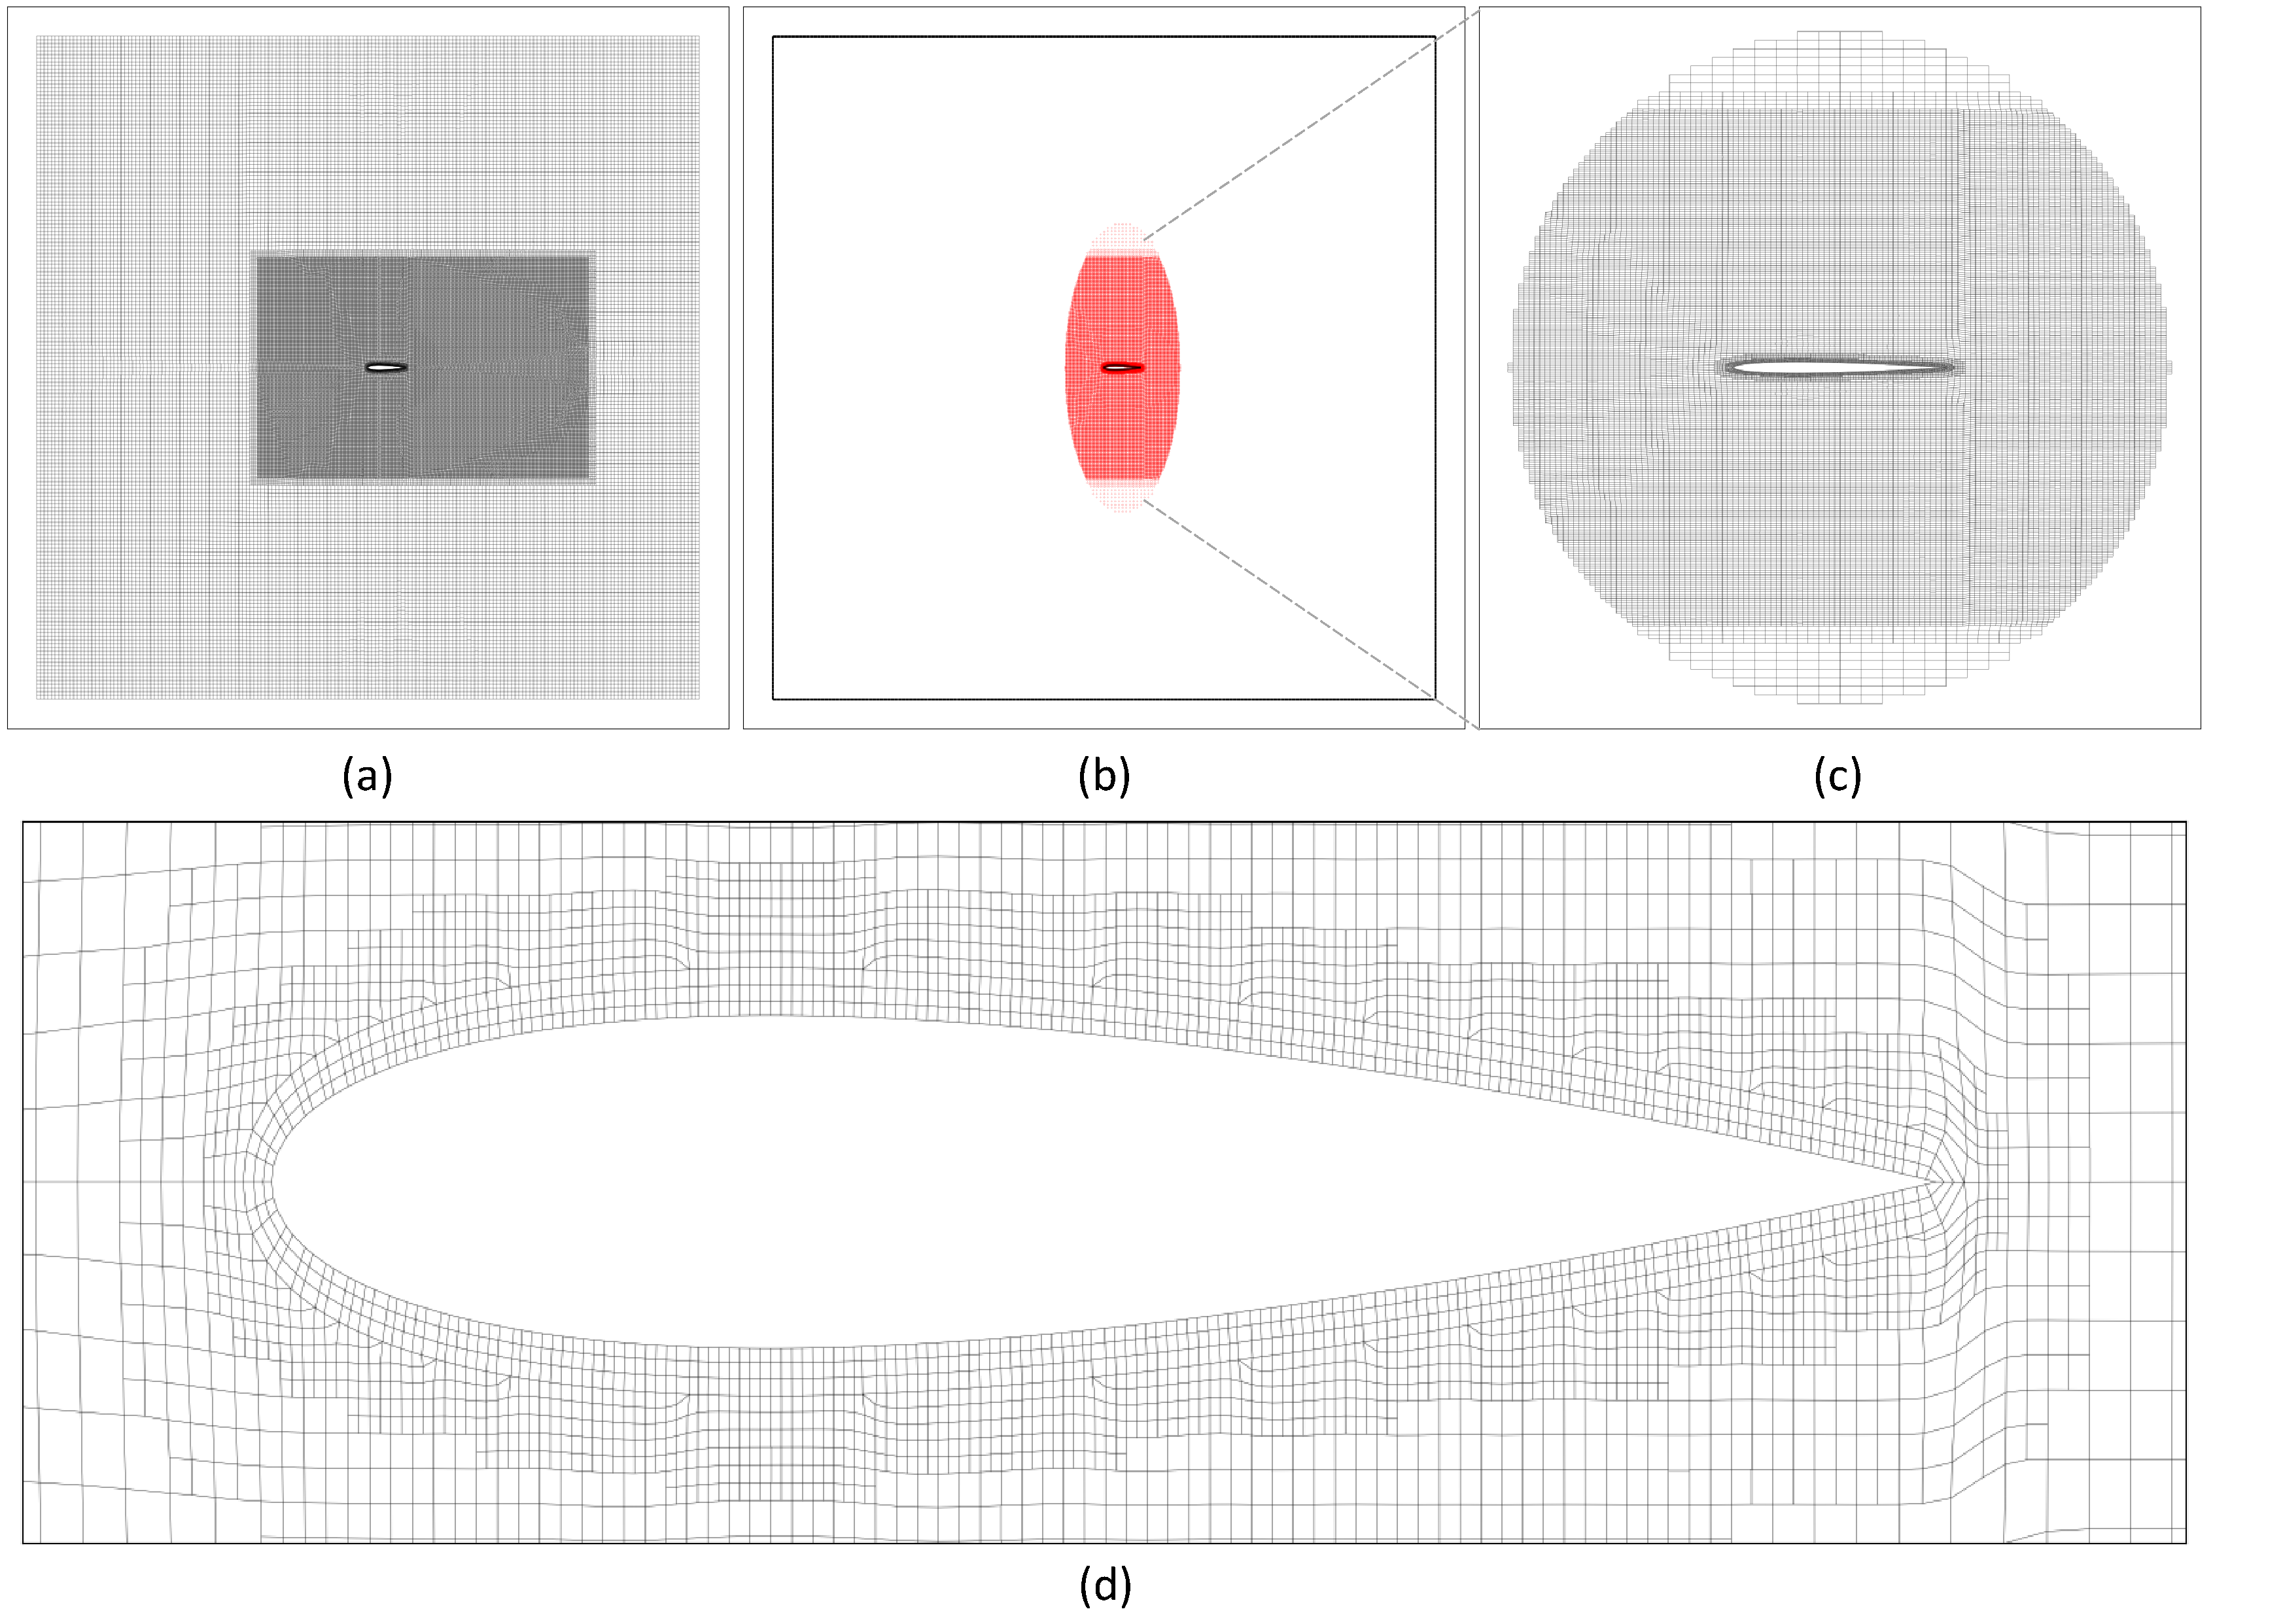
\includegraphics[width=1\linewidth]{chapter3/tex/figures/experiment/init_template_mesh_blockmesh.pdf}
	\end{center}
	\caption{ \small
		The template blockmesh TM-C with views of its (a) overall mesh, (b) boundary, (c) deformation area and (d) surface.
	}
	\label{ch3:fig:discuss_init_blockmesh}
\end{figure}

\begin{figure}[!htb]
	\begin{center}
		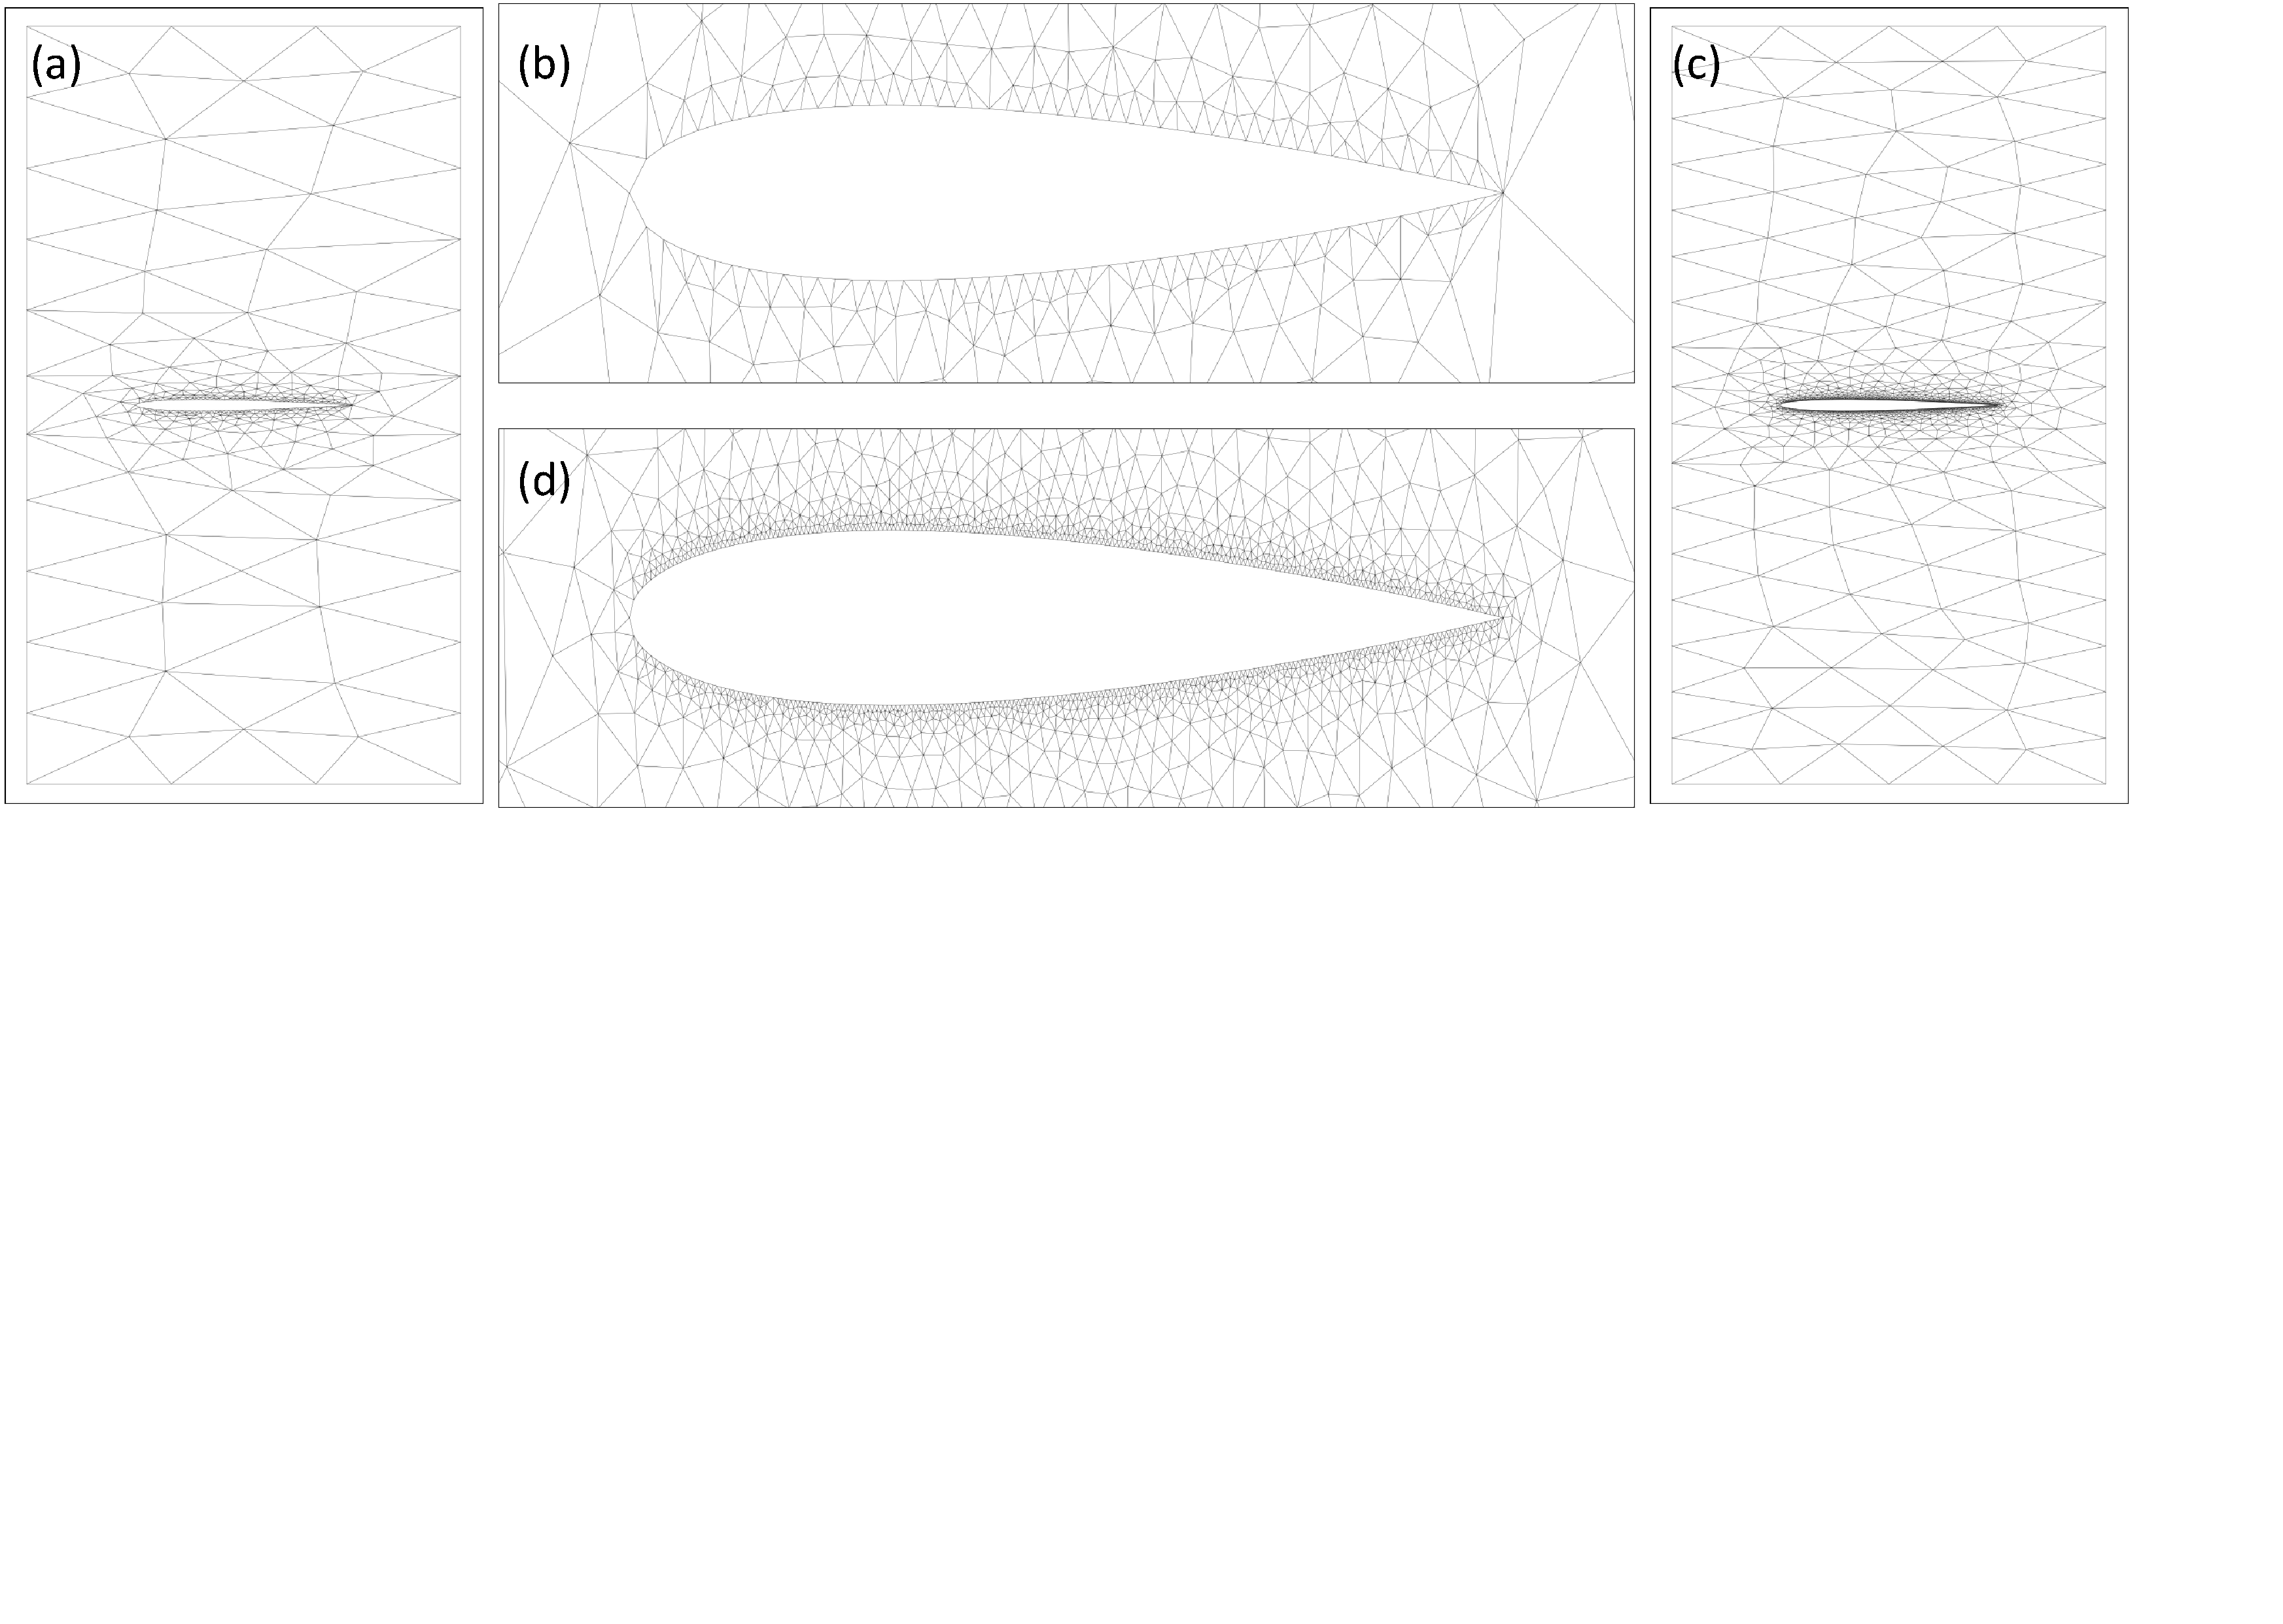
\includegraphics[width=1\linewidth]{chapter3/tex/figures/experiment/init_template_mesh_gmsh.pdf}
	\end{center}
	\caption{
		\small The (a-b) coarse and (c-d) fine triangulated template meshes generated by Gmsh.
	}
	\label{ch3:fig:discuss_init_gmsh}
\end{figure}

\begin{figure}[!htbp]
	\begin{center}
		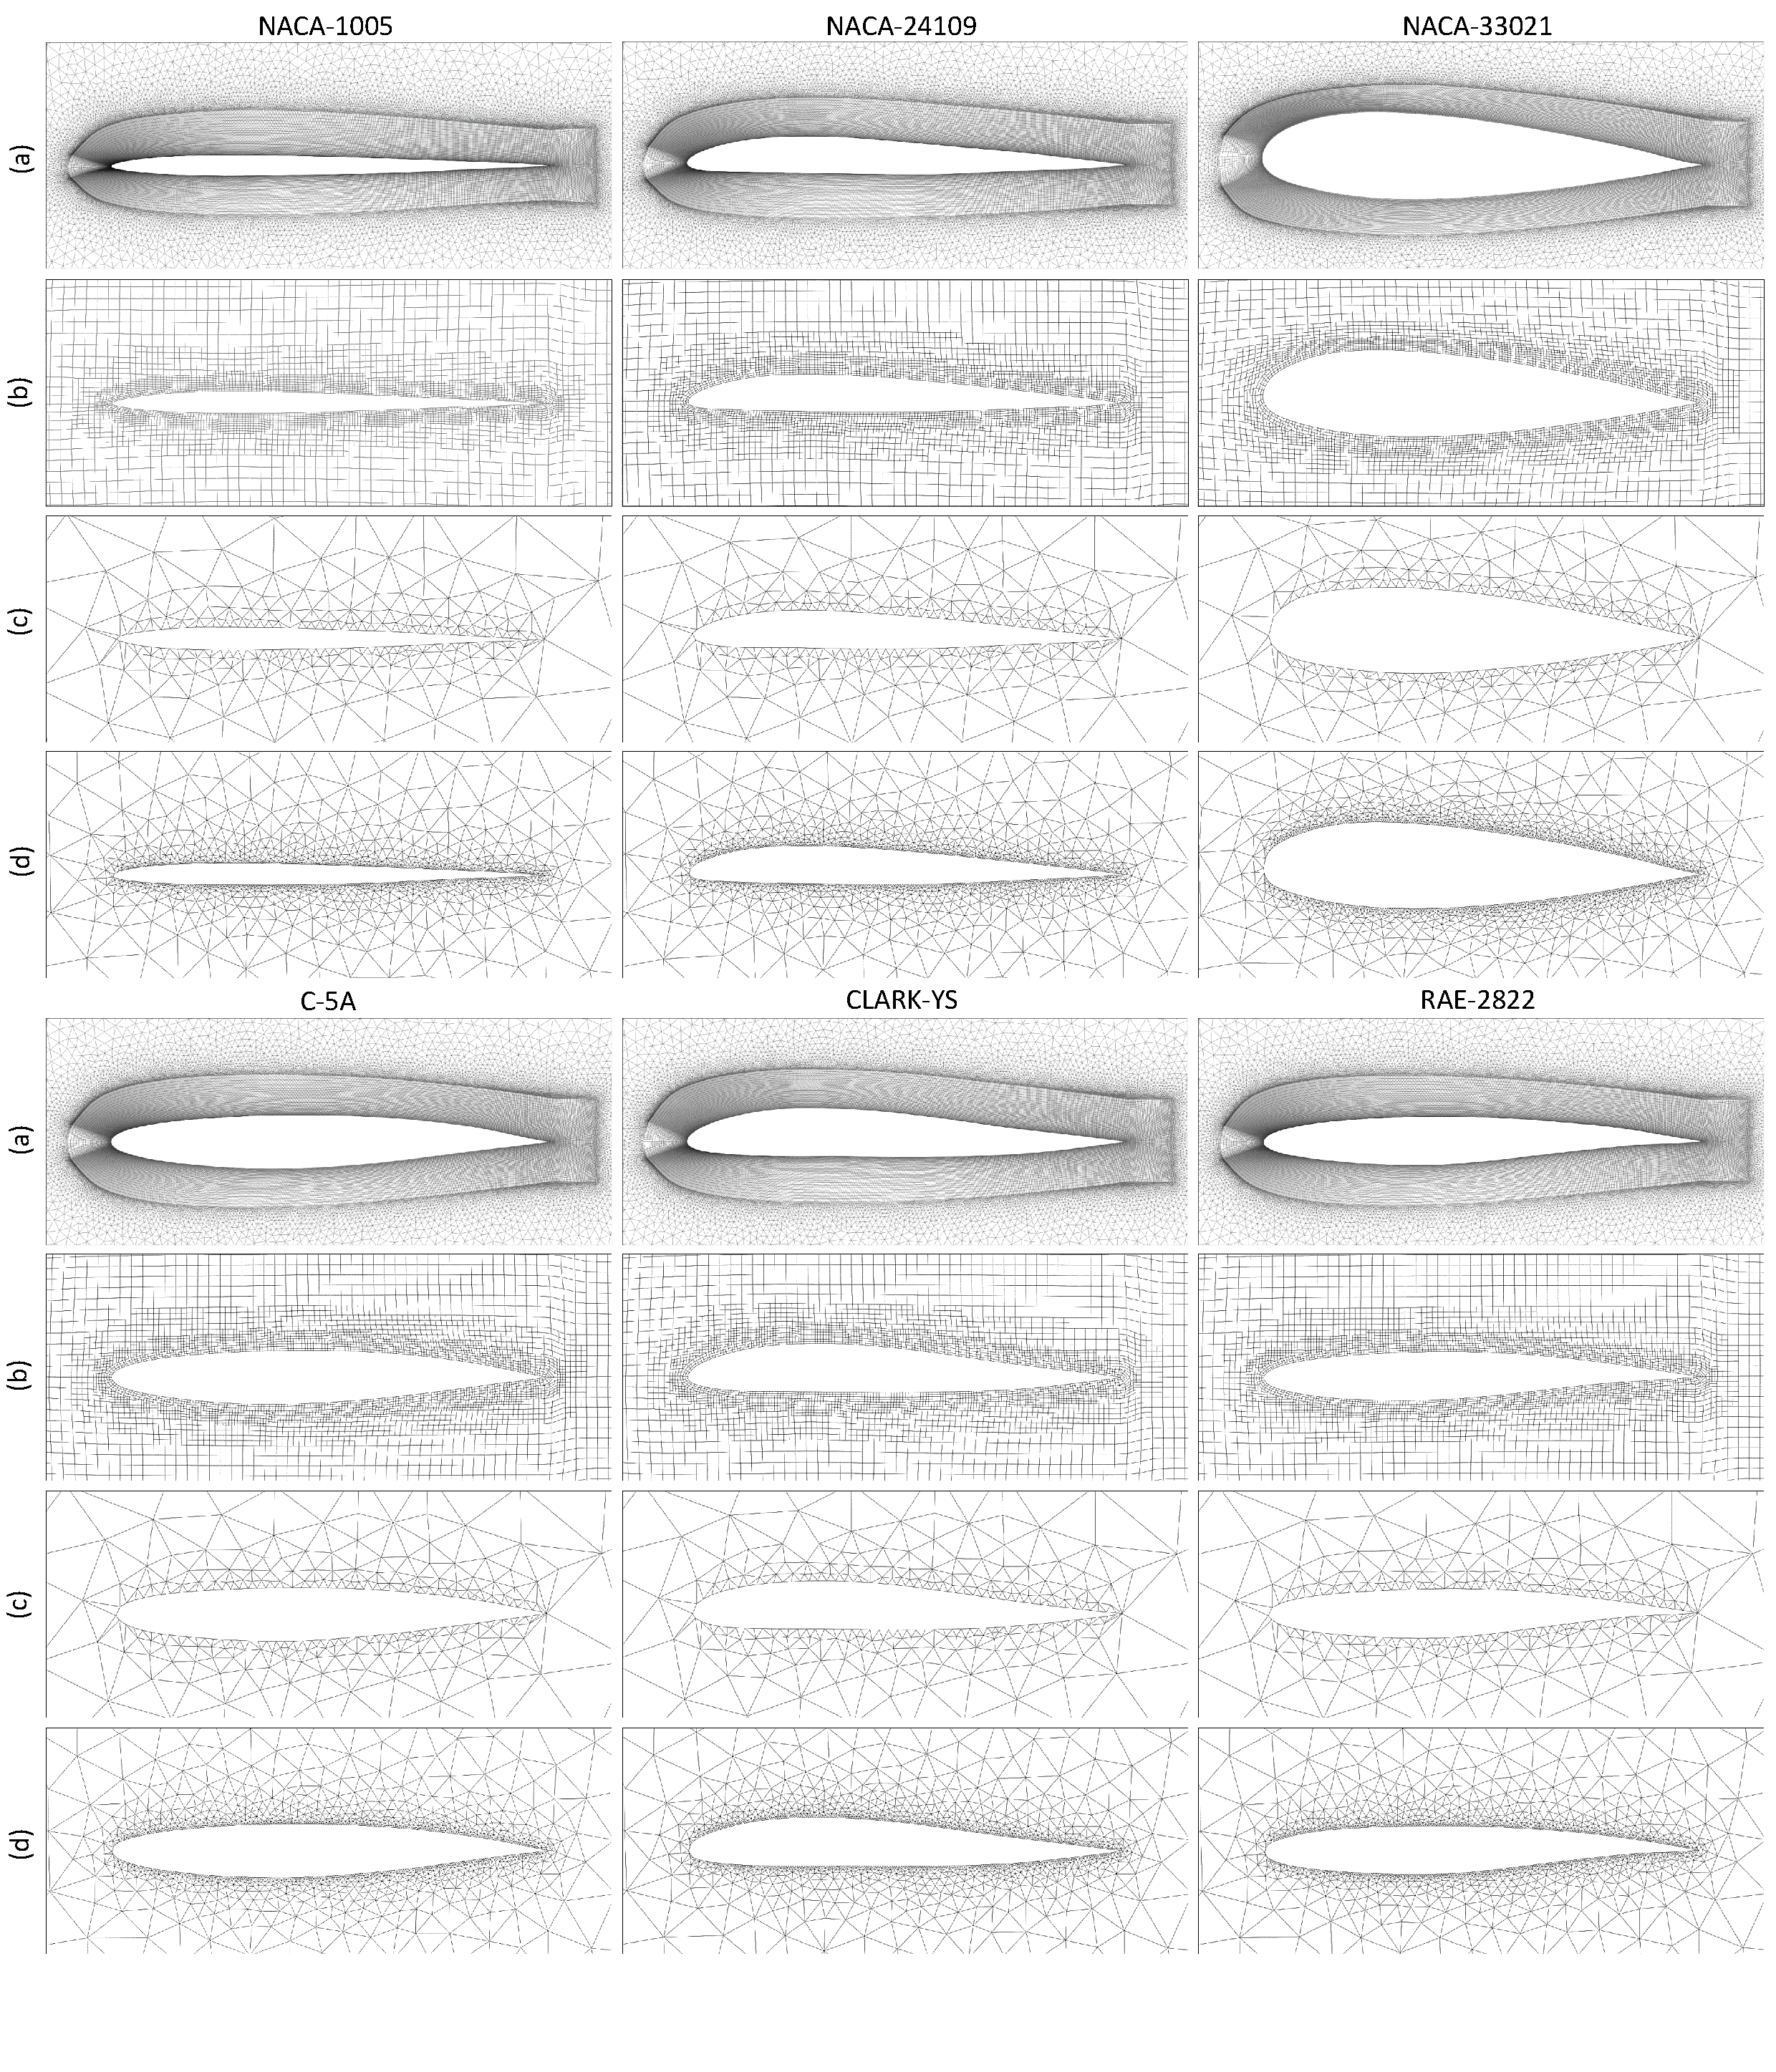
\includegraphics[width=1.02\linewidth]{chapter3/tex/figures/experiment/deformed_template_mesh.pdf}
	\end{center}
	\caption{
		\small Mesh reconstructions inferred with (a) TM-B, (b) TM-C, (c) TM-D1 and (c) TM-D2. Best viewed with zoom-in.
 	}
	\label{ch3:fig:discuss_template_res}
\end{figure}

\begin{itemize}
    \item {\textbf{The hybrid parametric mesh (denoted as TM-B)} is generated by VLab \cite{aa.Chappin2010, aa.Viola2018}, as shown in Fig.\ref{ch3:fig:discuss_init_vlab_mesh}. It comprises a triangulated part that divides the far field and well refined wall layers that fully resolves the boundary region. It contains $64,917$ vertices and $216,793$ edges belonging to triangles and rectangles.}

    \item \textbf{The block mesh (denoted as TM-C)} is generated by the OpenFoam's \textit{blockMesh} command on the NACA-0012 airfoil, as shown in Fig.\ref{ch3:fig:discuss_init_blockmesh}.
    The \textit{snappyHexMesh} options are used during meshing so that there are four mesh granularities and viscous layers, which leads to a mixture of cell types and various numbers of neighbors for vertices.
    Similar to TM-A, we also select a subarea surrounding the airfoil to deform.
    The deformation area contains 30,536 vertices and 29,848 polygon cells with 3, 4 or 5 edges.
    
    \item \textbf{The triangulation meshes} are generated by the Gmsh library \cite{aa.Geuzaine2009}.
    The cells are all triangulated.
    We use this meshing to studies the effect of different mesh densities.
    To do this, we create a coarse mesh (denoted as TM-D1) with 347 vertices and 564 faces (see Fig.\ref{ch3:fig:discuss_init_gmsh}(a)), and a fine mesh (denoted as TM-D2) with 1,642 vertices and 2,842 faces (see Fig.\ref{ch3:fig:discuss_init_gmsh}(b)).
    The overall mesh is relatively small so no subarea extraction is needed.
    The template airfoil is also NACA-0012.
\end{itemize}
%
Given these template meshes, TM-B is used for simulations in the following section, while TM-C, TM-D1 and TM-D2 are only used to investigating our model's generalization ability to different geometries.

Four random NACA airfoils and four random non-NACA airfoils are reconstructed using these different template meshes and Eq.\ref{ch3:eq:autodec}. No severe mesh quality issues are found in any of these results. 
A qualitative comparison near the airfoil is presented in Fig.\ref{ch3:fig:discuss_template_res} where the special structures created by the meshing algorithms in the template mesh are well preserved in all cases. The simulation results of Sec.\ref{ch3:sec:simulation} also indicate that meshes based on TM-B are of good quality.